\documentclass[conference]{IEEEtran}
\IEEEoverridecommandlockouts

\usepackage{cite}
\usepackage{amsmath,amssymb,amsfonts}
\usepackage{graphicx}
\usepackage{textcomp}
\usepackage{xcolor}
\usepackage{booktabs}
\usepackage{tikz}
\usepackage{pgfplots}
\pgfplotsset{compat=1.18}
\usetikzlibrary{arrows.meta,positioning,shapes.geometric,fit}
\def\BibTeX{{\rm B\kern-.05em{\sc i\kern-.025em b}\kern-.08em
    T\kern-.1667em\lower.7ex\hbox{E}\kern-.125emX}}

\begin{document}

\title{From Ensemble and DistilBERT Baselines to Deep Metric Learning:\\
An Extended Study for Imbalanced Windows PE Malware Detection}

\author{\IEEEauthorblockN{Ly Ngoc Vu}
\IEEEauthorblockA{\textit{Industrial University of Ho Chi Minh City} \\
Ho Chi Minh City, Vietnam \\
dezzhuge@gmail.com}
\and
\IEEEauthorblockN{Dang Thi Phuc}
\IEEEauthorblockA{\textit{Industrial University of Ho Chi Minh City} \\
Ho Chi Minh City, Vietnam \\
phucdt@iuh.edu.vn}}

\maketitle

\begin{abstract}
This paper extends a prior ATC 2024 study on Windows PE malware detection, which compared machine learning ensembles and text-based deep learning models (LSTM, BiLSTM, DistilBERT). The previous version achieved strong performance near 99\% accuracy on a large PE dataset. In this extended version, we add a deep metric learning (DML) branch on a unified Transformer backbone and evaluate five variants: baseline classification, ArcFace, Contrastive, Triplet, and Multi-Similarity. We report multi-seed statistics and low-false-positive operating behavior (TPR@FPR) for deployment-oriented analysis. Results show that DML is useful but objective-dependent: Multi-Similarity is strongest overall, while ArcFace is unstable under strict low-FPR operation.
\end{abstract}

\begin{IEEEkeywords}
malware detection, PE files, deep metric learning, Transformer, low-FPR evaluation
\end{IEEEkeywords}

\section{Introduction}
Malware detection on Windows PE files remains challenging under severe class imbalance and strict false-positive requirements. Prior experiments using classical ML and text-based deep learning showed strong aggregate accuracy. However, deployment effectiveness depends on behavior at strict operating points, not only global metrics.

This extension introduces deep metric learning (DML) objectives and compares them under a unified pipeline to assess both classification quality and low-FPR sensitivity.

\section{Relationship to Prior Work}
\subsection{Prior ATC 2024 Results}
The prior paper reported:
\begin{enumerate}
\item Classical ML models: Logistic Regression, Random Forest, SVC, XGBoost, plus ensemble voting/stacking.
\item Text-based deep learning models: LSTM, BiLSTM, DistilBERT.
\item Large PE dataset setting (\textasciitilde34k samples) with high performance.
\end{enumerate}

\subsection{Extension in This Paper}
This work adds:
\begin{enumerate}
\item Objective-level study of DML variants.
\item Multi-seed statistical evaluation.
\item Deployment-oriented low-FPR analysis.
\end{enumerate}

\section{Methodology}
A shared Transformer backbone is used, while objectives/heads vary:
\begin{enumerate}
\item baseline: cross-entropy/focal classification.
\item arcface: angular margin objective.
\item contrastive: pairwise distance objective + classification.
\item triplet: relative distance objective with hard mining.
\item multi\_similarity: weighted hard-pair similarity objective.
\end{enumerate}

\subsection{Pipeline Overview}
\begin{figure*}[!t]
\centering
\resizebox{\textwidth}{!}{%
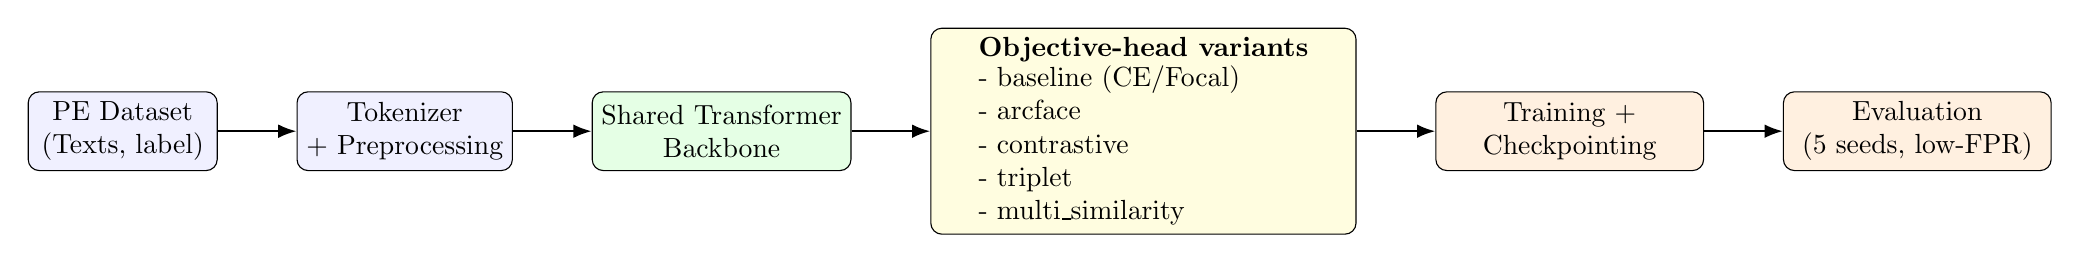
\begin{tikzpicture}[
    node distance=9mm and 10mm,
    stage/.style={draw, rounded corners, align=center, minimum height=10mm, minimum width=24mm, fill=blue!6},
    core/.style={draw, rounded corners, align=center, minimum height=10mm, minimum width=30mm, fill=green!10},
    block/.style={draw, rounded corners, align=left, minimum height=18mm, minimum width=54mm, fill=yellow!12},
    evalbox/.style={draw, rounded corners, align=center, minimum height=10mm, minimum width=34mm, fill=orange!12},
    arrow/.style={-Latex, thick}
]
    \node[stage] (data) {PE Dataset\\(Texts, label)};
    \node[stage, right=of data] (prep) {Tokenizer\\+ Preprocessing};
    \node[core, right=of prep] (backbone) {Shared Transformer\\Backbone};
    \node[block, right=of backbone] (heads) {\textbf{Objective-head variants}\\[-0.4mm]
        - baseline (CE/Focal)\\
        - arcface\\
        - contrastive\\
        - triplet\\
        - multi\_similarity};
    \node[evalbox, right=of heads] (train) {Training +\\Checkpointing};
    \node[evalbox, right=of train] (eval) {Evaluation\\(5 seeds, low-FPR)};

    \draw[arrow] (data) -- (prep);
    \draw[arrow] (prep) -- (backbone);
    \draw[arrow] (backbone) -- (heads);
    \draw[arrow] (heads) -- (train);
    \draw[arrow] (train) -- (eval);
\end{tikzpicture}}
\caption{Unified pipeline for baseline and DML variants.}
\label{fig:pipeline}
\end{figure*}

\section{Results}
\subsection{Prior ATC 2024 Baselines}
\begin{table}[htbp]
\caption{ML baselines from prior paper}
\centering
\footnotesize
\begin{tabular}{lcccc}
\toprule
Model & Precision & Recall & F1 & Accuracy \\
\midrule
Logistic Regression & 0.990086 & 0.990232 & 0.990111 & 0.990112 \\
Random Forest & 0.990000 & 0.990382 & 0.990402 & 0.990403 \\
SVC & 0.990000 & 0.988060 & 0.988075 & 0.988076 \\
XGBoost & 0.990000 & 0.991542 & 0.991566 & 0.991566 \\
\bottomrule
\end{tabular}
\label{tab:prior_ml}
\end{table}

\begin{table}[htbp]
\caption{Deep learning baselines from prior paper}
\centering
\footnotesize
\begin{tabular}{lcccc}
\toprule
Model & Precision & Recall & F1 & Accuracy \\
\midrule
DistilBERT & 0.9864895 & 0.9865220 & 0.9864705 & 0.986471 \\
LSTM & 0.9674135 & 0.9674490 & 0.9674130 & 0.967413 \\
BiLSTM & 0.9507005 & 0.9499545 & 0.9500705 & 0.950102 \\
\bottomrule
\end{tabular}
\label{tab:prior_dl}
\end{table}

\subsection{New DML Results}
\begin{table}[htbp]
\caption{Aggregated 5-seed metrics (mean)}
\centering
\scriptsize
\setlength{\tabcolsep}{3pt}
\resizebox{\columnwidth}{!}{%
\begin{tabular}{lccccc}
\toprule
Variant & Accuracy & F1 & ROC-AUC & PR-AUC & TPR@FPR=1e-2 \\
\midrule
baseline & 0.9924 & 0.9960 & 0.9983 & 0.9999 & 0.9754 \\
arcface & 0.7979 & 0.7934 & 0.9704 & 0.9984 & 0.0000 \\
contrastive & 0.9931 & 0.9964 & 0.9971 & 0.9997 & 0.9533 \\
triplet & 0.9932 & 0.9964 & 0.9969 & 0.9998 & 0.9351 \\
multi\_similarity & \textbf{0.9946} & \textbf{0.9972} & 0.9978 & 0.9999 & \textbf{0.9851} \\
\bottomrule
\end{tabular}
}
\label{tab:new_results}
\end{table}

\begin{figure}[htbp]
\centering
\includegraphics[width=\columnwidth]{figures/dml_acc_f1.png}
\caption{Accuracy and F1 across DML variants (5-seed mean).}
\label{fig:accf1}
\end{figure}

\begin{figure}[htbp]
\centering
\includegraphics[width=\columnwidth]{figures/dml_runtime.png}
\caption{Single-run runtime per variant.}
\label{fig:runtime}
\end{figure}

\begin{figure}[htbp]
\centering
\includegraphics[width=\columnwidth]{figures/dml_lowfpr.png}
\caption{Low-FPR sensitivity comparison; ArcFace is unstable at strict operating point.}
\label{fig:lowfpr}
\end{figure}

\section{Discussion}
Main findings:
\begin{enumerate}
\item DML helps, but improvements are objective-dependent.
\item Multi-Similarity is strongest overall in this setup.
\item Baseline remains highly competitive.
\item ArcFace requires further calibration/tuning for strict low-FPR deployment.
\end{enumerate}

\section{Conclusion}
This extended study confirms that text-based PE malware detection can achieve high performance and that DML can further improve deployment-oriented behavior when the objective is carefully selected. Multi-Similarity is the recommended candidate in the current experiments.

\section*{Acknowledgment}
This work extends the authors' prior ATC 2024 study and integrates new metric-learning experiments and analysis.

\begin{thebibliography}{00}
\bibitem{atc2024} L. N. Vu and D. T. Phuc, "Windows Malware Detection: Exploring from Machine Learning to Text-Based Deep Learning Approaches," in Proc. ATC, 2024.
\bibitem{arcface} J. Deng et al., "ArcFace: Additive Angular Margin Loss for Deep Face Recognition," CVPR, 2019.
\bibitem{msloss} X. Wang et al., "Multi-Similarity Loss with General Pair Weighting for Deep Metric Learning," CVPR, 2019.
\bibitem{triplet} F. Schroff et al., "FaceNet: A Unified Embedding for Face Recognition and Clustering," CVPR, 2015.
\bibitem{contrastive} R. Hadsell et al., "Dimensionality Reduction by Learning an Invariant Mapping," CVPR, 2006.
\end{thebibliography}

\end{document}
